
\begin{questions}

  
\question Your wardrobe consists of 5 shirts, 3 pairs of pants, and 17 bow ties.  How many different outfits can you make?

  \begin{answer}
    255.
  \end{answer}


  
\question For your college interview, you must wear a tie.  You own 3 regular (boring) ties and 5 (cool) bow ties.  How many choices do you have for your neck-wear? 

  \begin{answer}
    8.
  \end{answer}




\question You realize that the interview is for clown-college, so you should probably wear both a regular tie and a bow tie.  How many choices do you have now?

  \begin{answer}
    15.
  \end{answer}



\question You realize that it would also be okay to wear more than two ties.
\begin{parts}
 \part You must select some of your ties to wear - everything is okay, from no ties up to all ties.  How many choices do you have?
 \part If you want to wear at least one regular tie and one bow tie, but are willing to wear up to all your ties, how many choices do you have for which ties to wear?
 \part How many choices do you have if you wear exactly 2 of the 3 regular ties and 3 of the 5 bow ties?
 \part Once you have selected 2 regular and 3 bow ties, in how many orders could you put the ties on, assuming you must have one of the three bow ties on top?
\end{parts}

  \begin{answer}
    \begin{parts}
      \part $2^8 = 256$.  You have two choices for each tie - wear it or don't. %You must select some of your ties to wear - everything is okay, from no ties up to all ties.  How many choices do you have?
      \part You have 7 choices for regular ties (the 8 choices less the ``no regular tie'' option) and 31 choices for bow ties (32 total minus the ``no bow tie'' option).  Thus total you have $7 \cdot 31 = 217$.  %If you want to wear at least one regular tie and one bow tie, but are willing to wear up to all your ties, how many choices do you have for which ties to wear?
      \part ${3\choose 2}{5\choose 3} = 30$  %How many choices do you have if you wear exactly 2 of the 3 regular ties and 3 of the 5 bow ties?
      \part $5! = 120$  %Once you have selected 2 regular and 3 bow ties, in how many orders could you put the ties on, assuming you must have one of the three bow ties on top?
    \end{parts}
  \end{answer}



\question Your Blu-ray collection consists of 9 comedies and 7 horror movies. Give an example of a question for which the answer is:
\begin{parts}
 \part 16.
 \part 63.
\end{parts}

  \begin{answer}
    \begin{parts}
      \part 16 is the number of choices you have if you want to watch one movie, either a comedy or horror flick.
      \part 63 is the number of choices you have if you will watch two movies, first a comedy and then a horror.
    \end{parts}
  \end{answer}


  
\question If $|A| = 10$ and $|B| = 15$, what is the largest possible value for $|A \cap B|$?  What is the smallest?  What are the possible values for $|A \cup B|$?

  \begin{answer}
    $0 \le |A \cap B| \le 10$ and $15 \le |A \cup B| \le 25$.
  \end{answer}



\question If $|A| = 8$ and $|B| = 5$, what is $|A \cup B| + |A \cap B|$?

  \begin{answer}
      $|A \cup B| + |A \cap B| = 13$
  \end{answer}

  
  
  
\question A group of college students were asked about their TV watching habits.  Of those surveyed, 28 students watch {\em Elementary}, 19 watch {\em Castle} and 24 watch of {\em The Mentalist}.  Additionally, 16 watch {\em Elementary} and {\em Castle}, 14 watch {\em elementary} and {\em The Mentalist} and 10 watch {\em Castle} and {\em The Mentalist}.  There are 8 students who watch all three shows.  How many students surveyed watched at least one of the shows?

  \begin{answer}
    39.
  \end{answer}



\question Find $|(A \cup C)\cap \bar B|$ provided $|A| = 50$, $|B| = 45$, $|C| = 40$, $|A\cap B| = 20$, $|A \cap C| = 15$, $|B \cap C| = 23$ and $|A \cap B \cap C| = 12$.

    \begin{answer}
      $|(A \cup C)\cap \bar B| = 44$.  Use a Venn diagram.
    \end{answer}



\question Using the same data as the previous question, describe a set with cardinality 26.

    \begin{answer}
	One possibility: $(A \cup B) \cap C$.
    \end{answer}

    
    
\question Consider all 5 letter ``words'' made from the letters $a$ through $h$.
\begin{parts}
 \part How many of these words are there total?
 \part How many of these words contain no repeated letters?
 \part How many of these words (repetitions allowed) start with the sub-word ``aha''?
 \part How many of these words (repetitions allowed) either start with ``aha'' or end with ``bah'' or both?
 \part How many of the words containing no repeats also do not contain the sub-word ``bad'' (in consecutive letters)?  
\end{parts}

  \begin{answer}
    \begin{parts}
      \part $8^5$, since you select from 8 letters 5 times.  %How many of these words are there total?
      \part $P(8,5) = 8\cdot 7\cdot 6\cdot 5\cdot 4$.  After selecting a letter, you have fewer letters to select for the next one.  %How many of these words contain no repeated letters?
      \part 64 - you need to select the 4th and 5th letters. %How many of these words (repetitions allowed) start with the sub-word ``aha''?
      \part $64 + 64 - 0 = 128$.  There are 64 words which start with ``aha'' and another 64 words that end with ``bah.''  Perhaps we over counted the words that both start with ``aha'' and end with ``bah'' but since the words are only 5 letters long, there are no such words.  %How many of these words (repetitions allowed) either start with ``aha'' or end with ``bah'' or both?
      \part $P(8,5) - 3\cdot P(5,2) = 6660$ - all the words minus the bad ones.  The taboo word can be in any of three positions (starting with letter 1, 2, or 3) and for each position we must choose the other two letters (from the remaining 5 letters) %How many of the words containing no repeats also do not contain the sub-word ``bad'' (in consecutive letters)?  
    \end{parts}
  \end{answer}



\question How many 10-bit strings contain 6 or more 1's?

  \begin{answer}
    ${10 \choose 6} + {10\choose 7} + {10\choose 8} + {10 \choose 9} + {10\choose 10} = 386$ 
  \end{answer}



\question What is the coefficient of $x^9$ in the expansion of $(x+1)^{14} + x^3(x+2)^{15}$?

  \begin{answer}
    Use the binomial theorem.  ${14\choose 9} + {15 \choose 6}2^9$.
  \end{answer}



\question Let $S = \{1, 2, 3, 4, 5, 6\}$
\begin{parts}
  \part How many subsets are there total? 
  \part How many subsets contain $\{2,3,5\}$ as a subset?
  \part How many subsets of $S$ contain no prime numbers?
  \part How many subsets contain at least one odd number? 
  \part How many doubletons (i.e., subsets of two elements) contain exactly one even number?
\end{parts}

  \begin{answer}
    \begin{parts}
      \part $2^6 = 64$  %How many subsets are there total? 
      \part $2^3 = 8$.  We need to select yes/no for each of the remaining three elements.  %How many subsets contain $\{2,3,5\}$ as a subset?
      \part $2^3 = 8$.  We need to decide yes/no for the three non-prime elements.  %How many subsets of $S$ contain no prime numbers?
      \part $2^6 - 2^3 = 56$.  There are 8 subsets which do not contain any odd numbers. %How many subsets contain at least one odd number? 
      \part 9.  We need to select one odd (3 choices) and one even (3 choices).  %How many doubletons (i.e., subsets of two elements) contain exactly one even number?
    \end{parts}
  \end{answer}


   
\question How many shortest lattice paths start at (3,3) and
\begin{parts}
  \part end at (10,10)?
  \part end at (10,10) and pass through (5,7)?
  \part end at (10,10) and avoid (5,7)?
\end{parts}   

  \begin{answer}
    \begin{parts}
      \part ${14 \choose 7}$ %end at (10,10)?
      \part ${6 \choose 2}{8\choose 5}$ %end at (10,10) and pass through (5,7)?
      \part ${14 \choose 7} - {6\choose 2}{8 \choose 5}$ %end at (10,10) and avoid (5,7)?
    \end{parts} 
  \end{answer}


   
\question A pizza parlor offers 10 toppings.
\begin{parts}
 \part How many 3-topping pizzas could they put on their menu?  Assume double toppings are not allowed.
 \part How many total pizzas are possible, with between zero and ten toppings (but not double toppings) allowed?
 \part The pizza parlor will list the 10 toppings in two columns on their menu.  How many ways can they arrange the toppings in the left column?
\end{parts}

  \begin{answer}
    \begin{parts}
      \part ${10 \choose 3}$ %How many 3-topping pizzas could they put on their menu?  Assume double toppings are not allowed.
      \part $2^{10}$ %How many total pizzas are possible, with between zero and ten toppings (but not double toppings) allowed?
      \part $P(10,5)$  %The pizza parlor will list the 10 toppings in two columns on their menu.  How many ways can they arrange the toppings in the left column?
    \end{parts}
  \end{answer}



\question How many quadrilaterals can you draw using the dots below as vertices (corners)?

\begin{center}
 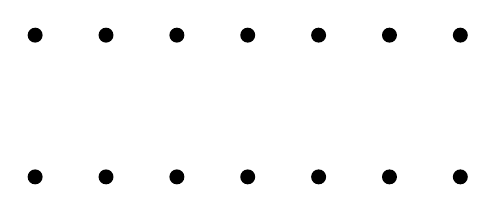
\begin{tikzpicture}[scale=.9]
  \foreach \x in {-3,...,3}
  \foreach \y in {-1,1}
  \fill (\x,\y) circle (3pt);
 \end{tikzpicture}
\end{center}

  \begin{answer}
    ${7\choose 2}{7\choose 2}$
  \end{answer}



\question How many of the quadrilaterals possible in the previous problem are:
\begin{multicols}{4}
\begin{parts}
 \part Squares?
 \part Rectangles?
 \part Parallelograms?
 \part Trapezoids?
\end{parts}
\end{multicols}

  \begin{answer}
    \begin{parts}
      \part 5 (you need to skip one dot the top and the bottom). %Squares?
      \part ${7 \choose 2}$ - once you select the two dots on the top, the bottom two are determined. % Rectangles?
      \part This is tricky - you need to worry about running out of space.  One way to count: break into cases by the location of the top left corner.  You get ${7 \choose 2} + ({7 \choose 2}-1) + ({7 \choose 2} - 3) + ({7 \choose 2} - 6) + ({7 \choose 2} - 10) + ({7 \choose 2} - 15)$ %Parallelograms?
      \part All of them %Trapezoids?
    \end{parts}
  \end{answer}




\question On a business retreat, your company of 20 businessmen go golfing.
\begin{parts}
 \part You need to divide up into foursomes (groups of 4 people): a first foursome, a second foursome, and so on.  How many ways can you do this?
 \part After all your hard work, you realize that in fact, you want each foursome to include one of the five CEO's.  How many ways can you do this?
\end{parts}

  \begin{answer}
    \begin{parts}
      \part ${20 \choose 4}{16 \choose 4}{12 \choose 4}{8 \choose 4}{4 \choose 4}$ %You need to divide up into foursomes (groups of 4 people): a first foursome, a second foursome, and so on.  How many ways can you do this?
      \part $5!{15 \choose 3}{12 \choose 3}{9 \choose 3}{6 \choose 3}{3 \choose 3}$ %After all your hard work, you realize that in fact, you want each foursome to include one of the five CEO's.  How many ways can you do this?
    \end{parts}
  \end{answer}



\question How many different seating arrangements are possible for King Arthur and his 9 knights around their round table?

  \begin{answer}
     $9!$ (there are 10 people seated around the table, but it does not matter where King Arthur sits, only who sits to his left, two seats to his left, and so on).
  \end{answer}



  
\question Give a combinatorial proof for the identity $1 + 2 + 3 + \cdots + n = {n+1 \choose 2}$. 
	
	\begin{answer}
	\begin{proof}
        \underline{Question}: How many subsets of $A = {1,2,3, \ldots, n+1}$ contain exactly two elements?
        
        \underline{Answer 1}: We must choose 2 elements from $n+1$ choices, so there are ${n+1 \choose 2}$ subsets.
        
        \underline{Answer 2}: We break this question down into cases, based on what the larger of the two elements in the subset is. The larger element can't be 1, since we need at least one element smaller than it.
        
        Larger element is 2: there is 1 choice for the smaller element.
        
        Larger element is 3: there are 2 choices for the smaller element.
        
        Larger element is 4: there are 3 choices for the smaller element.
        
        And so on.  When the larger element is $n+1$, there are $n$ choices for the smaller element.  Since each two element subset must be in exactly one of these cases, the total number of two element subsets is $1 + 2 + 3 + \cdots + n$.
        
        Answer 1 and answer 2 are both correct, so they must be equal.  Therefore
        \[1 + 2 + 3 + \cdots + n = {n+1 \choose 2}\]
       \end{proof}
	\end{answer}
	
	
	
\question A woman is getting married.  She has 15 best friends but can only select 6 of them to be her bride's maids, one of which needs to be her maid of honor.  How many ways can she do this?
\begin{parts}
 \part What if she first selects the 6 bride's maids, and then selects one of them to be the maid of honor?
 \part What if she first selects her maid of honor, and then 5 other bride's maids?
 \part Explain why $6 {15 \choose 6} = 15 {14 \choose 5}$.
\end{parts}
	
	\begin{answer}
		\begin{parts}
		 \part She has ${15 \choose 6}$ ways to select the 6 bride's maids, and then for each way, has 6 choices for the maid of honor.  Thus she has ${15 \choose 6}6$ choices.  %What if she first selects the 6 bride's maids, and then selects one of them to be the maid of honor?
		 \part She has 15 choices for who will be her maid of honor.  Then she needs to select 5 of the remaining 14 friends to be bride's maids, which she can do in ${14 \choose 5}$ ways.  Thus she has $15 {14 \choose 5}$ choices.  %What if she first selects her maid of honor, and then 5 other bride's maids?
		 \part We have answered the question (how many wedding parties can the bride choose from) in two ways.  The first way gives the left hand side of the identity and the second way gives the right hand side of the identity.  Therefore the identity holds. %Explain why $6 {15 \choose 6} = 15 {14 \choose 5}$.
		\end{parts}
	\end{answer}
	
	
	
\question Consider the bit strings in $\b B^6_2$ (bit strings of length 6 and weight 2).
\begin{parts}
 \part How many of those bit strings start with 1?
 \part How many of those bit strings start with 01?
 \part How many of those bit strings start with 001?
 \part Are there any other strings we have not counted yet?  Which ones, and how many are there?
 \part How many bit strings are there total in $\b B^6_2$?
 \part What binomial identity have you just given a combinatorial proof for?
\end{parts}
	
	\begin{answer}
		\begin{parts}
		 \part After the 1, we need to find a 5-bit string with one 1.  There are ${5 \choose 1}$ ways to do this. %How many of those bit strings start with 1?
		 \part ${4 \choose 1}$ (we need to pick 1 of the remaining 4 slots to be the second 1). %How many of those bit strings start with 01?
		 \part ${3 \choose 1}$ %How many of those bit strings start with 001?
		 \part Yes.  We still need strings starting with 0001 (there are ${2 \choose 1}$ of these) and strings starting 00001 (there is only ${1 \choose 1} = 1$ of these).  %Are there any other strings we have not counted yet?  Which ones, and how many are there?
		 \part ${6 \choose 2}$ %How many bit strings are there total in $\b B^6_2$?
		 \part An example of the Hockey Stick Theorem:  %What binomial identity have you just given a combinatorial proof for?
		 \[{1 \choose 1} + {2 \choose 1} + {3 \choose 1} + {4 \choose 1} + {5 \choose 1} = {6 \choose 2}\]
		\end{parts}
	\end{answer}
	
	
	

\question Let's count {\em ternary} digit strings - strings in which each digit can be 0, 1, or 2.
\begin{parts}
 \part How many ternary digit strings contain exactly $n$ digits?  
 \part How many ternary digit strings contain exactly $n$ digits and $n$ 2's.
 \part How many ternary digit strings contain exactly $n$ digits and $n-1$ 2's.  (Hint: where can you put the non-2 digit, and then what could it be?)
 \part How many ternary digit strings contain exactly $n$ digits and $n-2$ 2's.  (Hint: see previous hint)
 \part How many ternary digit strings contain exactly $n$ digits and $n-k$ 2's.
 \part How many ternary digit strings contain exactly $n$ digits and no 2's. (Hint: what kind of a string is this?)
 \part Use the above parts to give a combinatorial proof for the identity
 \[{n \choose 0} + 2{n \choose 1} + 2^2{n \choose 2} + 2^3{n \choose 3} + \cdots + 2^n{n \choose n} = 3^n\]
\end{parts}
	
	\begin{answer}
		\begin{parts}
		 \part $3^n$, since there are 3 choices for each of the $n$ digits.  %How many ternary digit strings contain exactly $n$ digits?  
		 \part $1$, since all the digits need to be 2's.  However, we might write this as ${n \choose 0}$.  %How many ternary digit strings contain exactly $n$ digits and $n$ 2's.
		 \part There are ${n \choose 1}$ places to put the non-2 digit.  That digit can be either a 0 or a 1, so there are $2{n \choose 1}$ such strings.  %How many ternary digit strings contain exactly $n$ digits and $n-1$ 2's.  (Hint: where can you put the non-2 digit, and then what could it be?)
		 \part We must choose two slots to fill with 0's or 1's.  There are ${n \choose 2}$ ways to do that.  Once the slots are picked, we have two choices for the first slot (0 or 1) and two choices for the second slot (0 or 1).  So there are a total of $2^2{n \choose 2}$ such strings. %How many ternary digit strings contain exactly $n$ digits and $n-2$ 2's.  (Hint: see previous hint)
		 \part There are ${n \choose k}$ ways to pick which slots don't have the 2's.  Then those slots can be filled in $2^k$ ways (0 or 1 for each slot).  So there are $2^k{n \choose k}$ such strings. %How many ternary digit strings contain exactly $n$ digits and $n-k$ 2's.
		 \part These strings contain just 0's and 1's - so they are bit strings.  There are $2^n$ bit strings.  But keeping with the pattern above, we might write this as $2^n {n \choose n}$. %How many ternary digit strings contain exactly $n$ digits and no 2's. (Hint: what kind of a string is this?)
		 \part We answer the question of how many length $n$ ternary digit strings there are in two ways.  First, each digit can be one of three choices, so the total number of strings is $3^n$.  On the other hand, we could break the question down into cases by how many of the digits are 2's.  If they are all 2's, then there are ${n \choose 0}$ strings.  If all but one is a 2, then there are $2{n \choose 1}$ strings.  If all but 2 of the digits are 2's, then there are $2^2{n \choose 2}$ strings - we choose 2 of the $n$ digits to be non-2, and then there are 2 choices for each of those digits.  And so on for every possible number of 2's in the string.  %Use the above parts to give a combinatorial proof for the identity
		 %\[{n \choose 0} + 2{n \choose 1} + 2^2{n \choose 2} + 2^3{n \choose 3} + \cdots + 2^n{n \choose n} = 3^n\]
		\end{parts}
	\end{answer}
	
	
	
\question Give a combinatorial proof for the identity $P(n,k) = {n \choose k}k!$
	
	\begin{answer}
		\begin{proof}
         \underline{Question}: How many $k$-letter words can you make using $n$ different letters without repeating any letter?
         
         \underline{Answer 1}: There are $n$ choices for the first letter, $n-1$ choices for the second letter, $n-2$ choices for the third letter, and so on until $n - (k-1)$ choices for the $k$th letter (since $k-1$ letters have already been assigned at that point).  The product of these numbers can be written $\frac{n!}{(n-k)!}$ which is $P(n,k)$.
         
         \underline{Answer 2}: First pick $k$ letters to be in the word from the $n$ choices.  This can be done in ${n \choose k}$ ways.  Now arrange those letters into a word - there are $k$ choices for the first letter, $k-1$ choices for the second, and so on, for a total of $k!$ arrangements of the $k$ letters.  Thus the total number of words is ${n \choose k}k!$.
        \end{proof}
	\end{answer}
	
	
	
	
	
\question After gym class you are tasked with putting the 14 identical dodge-balls away into 5 bins.  
\begin{parts}
  \part How many ways can you do this if there are no restrictions?
  \part How many ways can you do this if each bin must contain at least one dodge-ball?
  \part How many ways can you do this if no bin can hold more than 6 balls?
\end{parts}

	\begin{answer}
	 \begin{parts}
	   \part ${18 \choose 4}$.  Each outcome can be represented by a sequence of 14 stars and 4 bars. %How many ways can you do this if there are no restrictions?
	   \part ${13 \choose 4}$.  First put one ball in each bin.  This leaves 9 stars and 4 bars.%How many ways can you do this if each bin must contain at least one dodge-ball?
	   \part ${18 \choose 4} - \left[ {5 \choose 1}{11 \choose 4} - {5 \choose 2}{4 \choose 4}\right]$.  Subtract all the distributions for which one or more bins contain 7 or more balls.  %How many ways can you do this if no bin can hold more than 6 balls?
	 \end{parts}
	\end{answer}
	
	


\question How many integer solutions are there to the equation $x + y + z = 8$
for which
\begin{parts}
  \part $x$, $y$, and $z$ are all positive?
  \part $x$, $y$, and $z$ are all non-negative?
  \part $x$, $y$, and $z$ are all greater than $-3$.
\end{parts}

	\begin{answer}
	\begin{parts}
	  \part ${7 \choose 2}$.  After each variable gets 1 star for free, we are left with 5 stars and 2 bars.  %$x$, $y$, and $z$ are all positive?
	  \part ${10 \choose 2}$.  We have 8 stars and 2 bars.  %$x$, $y$, and $z$ are all non-negative?
	  \part ${19 \choose 2}$.  This problem is equivalent to finding the number of solutions to $x' + y' + z' = 17$ where $x'$, $y'$ and $z'$ are non-negative.  (In fact, we really just do a substitution.  Let $x = x'- 3$, $y = y' - 3$ and $z = z' - 3$).  %$x$, $y$, and $z$ are all greater than $-3$.
	\end{parts}
	\end{answer}
	
	


\question When playing Yahtzee, you roll five regular 6-sided dice.  How many different outcomes are possible from a single roll?  The order of the dice does not matter.

	\begin{answer}
	${10 \choose 5}$.  We have 5 stars (the five dice) and 5 bars (the five switches between the number 1-6).
	\end{answer}
	
	


\question How many integer solutions to $x_1 + x_2 + x_3 + x_4  = 25$ are there fore which $x_1 \ge 1$, $x_2 \ge 2$, $x_3 \ge 3$  and $x_4 \ge 4$?

	\begin{answer}
	${18 \choose 3}$.  Distribute 10 units to the variables before finding all solutions to $x_1' + x_2' + x_3' + x_4' = 15$ in non-negative integers.
	\end{answer}
	
	


\question Write out all functions $f: \{1,2,3\}$ to $\{a,b\}$.  How many are there?  How many are injective?  How many are surjective?  How many are both?

	\begin{answer}
	There are 8 different functions.  For example, $f(1) = a$, $f(2) = a$, $f(3) = a$; or $f(1) = a$, $f(2) = b$, $f(3) = a$, and so on.  None of the functions are injective.  Exactly 6 of the functions are surjective.  No functions are both (since no functions here are injective).
	\end{answer}
	
	
	

\question Write out all functions $f: \{1,2\}$ to $\{a,b,c\}$.  How many are there?  How many are injective?  How many are surjective?  How many are both?

	\begin{answer}
	There are nine functions - you have a choice of three outputs for $f(1)$, and for each, you have three choices for the output $f(2)$.  Of these functions, 6 are injective, 0 are surjective, and 0 are both.
	\end{answer}
	
	
	

\question Consider the function $f:\{1,2,3,4,5\} \to \{1,2,3,4\}$ given by the table below:

\begin{center}
\begin{tabular}{c||c|c|c|c|c}
              $x$ & 1 & 2 & 3 & 4 & 5 \\ \hline
              $f(x)$ & 3 & 2 & 4 & 1 & 2
            \end{tabular}
\end{center}

\begin{parts}
  \part Is $f$ injective?  Explain.
  \part Is $f$ surjective?  Explain.
\end{parts}

	\begin{answer}
		\begin{parts}
		%Is $f$ injective?  Explain.
		\part $f$ is not injective, since $f(2) = f(5)$ - two different inputs have the same output. 
		% Is $f$ surjective?  Explain.
		\part $f$ is surjective, since every element of the codomain is an element of the range.
		\end{parts}
	\end{answer}
	
	
	

\question Consider the function $f:\{1,2,3,4\} \to \{1,2,3,4\}$ given by the graph below.
\begin{multicols}{2}
\begin{center}
  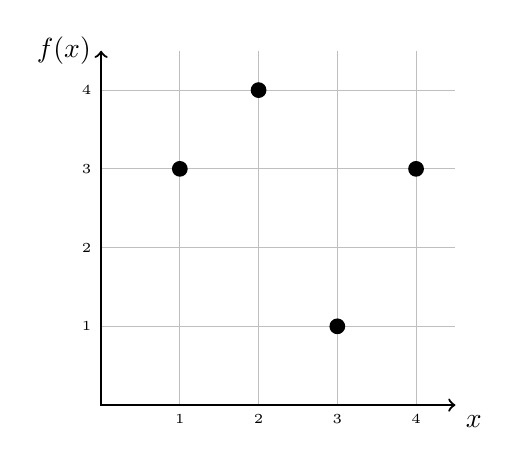
\begin{tikzpicture}[scale=1]
    \draw[thin, gray!50] (0,0) grid (4.5, 4.5);
    \draw[<->, thick] (0,4.5) node[left] {$f(x)$} -- (0,0) -- (4.5,0) node[below right] {$x$};
    \foreach \x in {1,2,3,4}
      \draw (\x,0) node[below] {\tiny \x} (0, \x) node[left] {\tiny \x};
    \fill (1,3) circle (.1) (2,4) circle (.1) (3,1) circle (.1) (4,3) circle (.1);
  \end{tikzpicture}
\end{center}

\begin{parts}
  \part Is $f$ injective?  Explain.
  \part Is $f$ surjective?  Explain.
\end{parts}
\end{multicols}


	\begin{answer}
		\begin{parts}
		%Is $f$ injective?  Explain.
		  \part $f$ is not injective, since $f(1) = 3$ and $f(4) = 3$.
		%   Is $f$ surjective?  Explain.
		  \part $f$ is not surjective, since there is no input which gives 2 as an output.
		\end{parts}
	\end{answer}
	
	
	


\question For each function given below, determine whether or not the function is injective and whether or not the function is surjective.
\begin{parts}
  \part $f:\N \to \N$ given by $f(n) = n+4$.
  \part $f:\Z \to \Z$ given by $f(n) = n+4$.
  \part $f:\Z \to \Z$ given by $f(n) = 5n - 8$.
  \part $f:\Z \to \Z$ given by $f(n) = \begin{cases}
                                         n/2 & \mbox{ if $n$ is even}\\
                                         (n+1)/2 & \mbox{ if $n$ is odd}.
                                       \end{cases}$
\end{parts}

	\begin{answer}
		\begin{parts}
		% $f:\N \to \N$ given by $f(n) = n+4$.
		  \part $f$ is injective, but not surjective.
		%   $f:\Z \to \Z$ given by $f(n) = n+4$.
		  \part $f$ is injective and surjective.
		  %$f:\Z \to \Z$ given by $f(n) = 5n - 8$.
		  \part $f$ is injective, but not surjective.
		%   $f:\Z \to \Z$ given by $f(n) = \begin{cases}
		%                                          n/2 & \mbox{ if $n$ is even}\\
		%                                          (n+1)/2 & \mbox{ if $n$ is odd}.
		%                                        \end{cases}$
		 \part $f$ is not injective, but is surjective.
		\end{parts}
	\end{answer}
	
	
	

%\question Let $A = \{1,2,3,\ldots,10\}$.  Consider the function $f:\pow(A) \to \N$ given by $f(B) = |B|$.  So $f$ takes a subset of $A$ as an input and outputs the cardinality of that set.  
%\begin{parts}
%  \part Is $f$ injective?  Prove your answer.
%  \part Is $f$ surjective?  Prove your answer.
%  \part Find $f\inv(1)$.
%  \part Find $f\inv(0)$.
%  \part Find $f\inv(12)$.
%\end{parts}
%
%	\begin{answer}
%		\begin{parts}
%		% Is $f$ injective?  Prove your answer.
%		  \part $f$ is not injective.  To prove this, we must simply find two different elements of the domain which map to the same element of the codomain.  Since $f(\{1\}) = 1$ and $f(\{2\}) = 1$, we see that $f$ is not injective.
%		%   Is $f$ surjective?  Prove your answer.
%		  \part $f$ is not surjective.  The largest subset of $A$ is $A$ itself, and $|A| = 10$.  So no natural number greater than 10 will ever be an output.
%		%   Find $f\inv(1)$.
%		  \part $f\inv(1) = \{\{1\}, \{2\}, \{3\}, \ldots \{10\}\}$ (the set of all the singleton subsets of $A$).
%		%   Find $f\inv(0)$.
%		  \part $f\inv(0) = \{\emptyset\}$.  Note, it would be wrong to write $f\inv(0) = \emptyset$ - that would claim that there is no input which has 0 as an output.
%		   % Find $f\inv(12)$.
%		  \part $f\inv(12) = \emptyset$, since there are no subsets of $A$ with cardinality 12.
%		\end{parts}
%	\end{answer}
	
	
	

%\question Let $A = \{n \in \N \st 0 \le n \le 999\}$ be the set of all numbers with three or fewer digits.  Define the function $f:A \to \N$ by $f(abc) = a+b+c$, where $a$, $b$, and $c$ are the digits of the number in $A$.  For example, $f(253) = 2 + 5 + 3 =  10$.
%\begin{parts}
%  \part Find $f\inv(3)$.
%  \part Find $f\inv(28)$.
%  \part Use one of the parts above to prove that $f$ is not injective.
%  \part Use one of the parts above to prove that $f$ is not surjective.
%\end{parts}
%
%	\begin{answer}
%		\begin{parts}
%		% Find $f\inv(3)$.
%		  \part $f\inv(3) = \{003, 030, 300, 012, 021, 102, 201, 120, 210, 111\}$
%		%   Find $f\inv(28)$.
%		  \part $f\inv(28) = \emptyset$ (since the largest sum of three digits is $9+9+9 = 27$)
%		%   Use one of the parts above to prove that $f$ is not injective.
%		  \part Part (a) proves that $f$ is not injective - the output 3 is assigned to 10 different inputs.
%		%   Use one of the parts above to prove that $f$ is not surjective.
%		  \part Part (b) proves that $f$ is not surjective - there is an element of the codomain (28) which is assigned to no inputs.
%		\end{parts}
%	\end{answer}
	
	
	

%\question Find a set $X$ and a function $f:X \to \N$ so that $f\inv(0) \cup f\inv(1) = X$.
%
%	\begin{answer}
%		$X$ can really be any set, as long as $f(x) = 0$ or $f(x) = 1$ for every $x \in X$.  For example, $X = \N$ and $f(n) = 0$ works.
%	\end{answer}
	
	
	

\question What can you deduce about the sets $X$ and $Y$ if you know,
\begin{parts}
  \part there is a injective function $f:X \to Y$.  Explain.
  \part there is a surjective function $f:X \to Y$.  Explain.
  \part there is a bijection $f:X \to Y$.  Explain.
\end{parts}

	\begin{answer}
		\begin{parts}
		% there is a injective function $f:X \to Y$.  Explain.
		  \part $|X| \le |Y|$ - otherwise two or more of the elements of $X$ would need to map to the same element of $Y$.
		%   there is a surjective function $f:X \to Y$.  Explain.
		  \part $|X| \ge |Y|$ - otherwise there would be one or more elements of $Y$ which were never an output.
		%   there is a bijection $f:X \to Y$.  Explain.
		  \part $|X| = |Y|$.  This is the only way for both of the above to occur.
		\end{parts}
	\end{answer}
	
	
	

\question Suppose $f:X \to Y$ is a function.  Which of the following are possible?  Explain.
\begin{parts}
  \part $f$ is injective but not surjective.
  \part $f$ is surjective but not injective.
  \part $|X| = |Y|$ and $f$ is injective but not surjective.
  \part $|X| = |Y|$ and $f$ is surjective but not injective.
  \part $|X| = |Y|$, $X$ and $Y$ are finite, and $f$ is injective but not surjective.
  \part $|X| = |Y|$, $X$ and $Y$ are finite, and $f$ is surjective but not injective.
\end{parts}

	\begin{answer}
		\begin{parts}
		% $f$ is injective but not surjective.
		  \part Yes. (Can you give an example?)
		  \part Yes. %$f$ is surjective but not injective.
		  \part Yes. %$|X| = |Y|$ and $f$ is injective but not surjective.
		  \part Yes. %$|X| = |Y|$ and $f$ is surjective but not injective.
		  \part No. %$|X| = |Y|$, $X$ and $Y$ are finite, and $f$ is injective but not surjective.
		  \part No. %$|X| = |Y|$, $X$ and $Y$ are finite, and $f$ is surjective but not injective.
		\end{parts}
	\end{answer}
	
	
	

%\question Consider the function $f:\Z \to \Z$ given by $f(n) = \begin{cases}
%                                                                 n+1 & \mbox{ if $n$ is even}\\
%                                                                 n-3 & \mbox{ if $n$ is odd}.
%                                                               \end{cases}$
%\begin{parts}
%  \part Is $f$ injective?  Prove your answer.
%  \part Is $f$ surjective?  Prove your answer.
%\end{parts}
%
%	\begin{answer}
%		\begin{parts}
%		% Is $f$ injective?  Prove your answer.
%		  \part $f$ is injective. 
%		  \begin{proof}
%		   Let $x$ and $y$ be elements of the domain $\Z$.  Assume $f(x) = f(y)$.  If $x$ and $y$ are both even, then $f(x) = x+1$ and $f(y) = y+1$.  Since $f(x) = f(y)$, we have $x + 1 = y + 1$ which implies that $x = y$.  Similarly, if $x$ and $y$ are both odd, then $x - 3 = y-3$ so again $x = y$.  The only other possibility is that $x$ is even an $y$ is odd (or visa-versa).  But then $x + 1$ would be odd and $y - 3$ would be even, so it cannot be that $f(x) = f(y)$.  Therefore if $f(x) = f(y)$ we then have $x = y$, which proves that $f$ is injective.
%		  \end{proof}
%		% Is $f$ surjective?  Prove your answer.
%		  \part $f$ is surjective.
%		  \begin{proof}
%		   Let $y$ be an element of the codomain $\Z$.  We will show there is an element $n$ of the domain ($\Z$) such that $f(n) = y$.  There are two cases.  First, if $y$ is even, then let $n = y+3$.  Since $y$ is even, $n$ is odd, so $f(n) = n-3 = y+3-3 = y$ as desired.  Second, if $y$ is odd, then let $n = y-1$.  Since $y$ is odd, $n$ is even, so $f(n) = n+1 = y-1+1 = y$ as needed.  Therefore $f$ is surjective.
%		  \end{proof}
%		
%		\end{parts}
%	\end{answer}
	
	
	


\question Consider functions $f: \{1,2,3,4\} \to \{a,b,c,d,e,f\}$.
\begin{parts}
  \part How many functions are there total?
  \part How many functions are injective?
  \part How many functions are surjective?
  \part How many functions have the property that $f(1) \ne a$ or $f(2) \ne b$, or both?
\end{parts}

	\begin{answer}
	\begin{parts}
	  \part $6^4 = 1296$, since there are six choices of where to send each of the 4 elements of the domain. %How many functions are there total?
	  \part $P(6, 4) = 6 \cdot 5 \cdot 4 \cdot 3 = 360$, since outputs cannot be repeated.  %How many functions are injective?
	  \part None. %How many functions are surjective?
	  \part There are $5 \cdot 6^3$ functions for which $f(1) \ne a$ and another $5 \cdot 6^3$ functions for which $f(2) \ne b$.  There are $5^2 \cdot 6^2$ functions for which both $f(1) \ne a$ and $f(2) \ne b$.  So the total number of functions for which $f(1) \ne a$ or $f(2) \ne b$ or both is
	  \[5 \cdot 6^3 + 5 \cdot 6^3 - 5^2 \cdot 6^2 = 1260\] %How many functions have the property that $f(1) \ne a$ or $f(2) \ne b$, or both?
	\end{parts}
	\end{answer}
	
	

\question Consider sets $A$ and $B$ with $|A| = 10$ and $|B| = 17$.
\begin{parts}
  \part How many functions $f: A \to B$ are there?
  \part How many functions $f: A \to B$ are injective?
\end{parts}

	\begin{answer}
	\begin{parts}
	  \part $17^{10}$ %How many functions $f: A \to B$ are there?
	  \part $P(17, 10)$  %How many functions $f: A \to B$ are injective?
	\end{parts}
	\end{answer}
	
	



\question Consider sets $A$ and $B$ with $|A| = 10$ and $|B| = 5$.  How many functions $f: A \to B$ are surjective?

	\begin{answer}
	$5^{10} - \left[{5 \choose 1}4^{10} - {5 \choose 2}3^{10} + {5 \choose 3}2^{10} - {5 \choose 4}1^{10}\right]$ %Consider sets $A$ and $B$ with $|A| = 10$ and $|B| = 5$.  How many functions $f: A \to B$ are surjective?
	\end{answer}
	
	


\question Let $A = \{1,2,3,4,5\}$.  How many injective functions $f:A \to A$ have the property that for each $x \in A$, $f(x) \ne x$?

	\begin{answer}
	$5! - \left[{5 \choose 1}4! - {5 \choose 2}3! + {5 \choose 3}2! - {5 \choose 4}1! + {5 \choose 5}0!\right]$.  This is a sneaky way to as for the number of derangements on 5 elements. %Let $A = \{1,2,3,4,5\}$.  How many injective functions $f:A \to A$ have the property that for each $x \in A$, $f(x) \ne x$?
	\end{answer}
	
	


\question Ten ladies of a certain age drop off their red hats at the hat check of a museum.  As they are leaving, the hat check attendant gives the hats back randomly.  In how many ways can exactly six of the ladies receive their own hat (and the other four not)?

	\begin{answer}
	${10 \choose 6}\left(4! - \left[{4 \choose 1} 3! - {4 \choose 2}2! + {4 \choose 3}1! - {4 \choose 4}0!\right]\right)$.  We choose 6 of the 10 ladies to get their own hat, and the multiply by the number of ways the remaining hats can be deranged. 
	\end{answer}
	
	



	


\question You have 9 presents to give to your 4 kids.  How many ways can this be done if
\begin{parts}
  \part The presents are identical, and each kid gets at least one present?
  \part The presents are identical, and some kids might get no presents?
  \part The presents are unique, and some kids might get no presents?
  \part the presents are unique and each kid gets at least one present?
\end{parts}

	\begin{answer}
	\begin{parts}
	  \part ${8 \choose 3}$, after giving one present to each kid, you are left with 5 presents (stars) which need to be divide among the 4 kids (giving 3 bars). %The presents are identical, and each kid gets at least one present?
	  \part ${12 \choose 3}$.  You have 9 stars and 3 bars.  %The presents are identical, and some kids might get no presents?
	  \part $4^9$.  You have 4 choices for whom to give each present.  This is like making a function from the set of present to the set of kids. %The presents are unique, and some kids might get no presents?
	  \part $4^9 - \left[{4 \choose 1}3^9 - {4\choose 2}2^9 + {4 \choose 3}1^9 \right]$.  Now the function from the set of present to the set of kids must be surjective. %the presents are unique and each kid gets at least one present?
	\end{parts}
	\end{answer}
	
	


\newpage

\question For each of the following counting problems, say whether the answer is


\begin{itemize}
\begin{multicols}{3}
  \item[A] ${10\choose 4}$
  \item[B] $P(10,4)$
  \item[C] Neither
  \end{multicols}
\end{itemize}

If you answer is ``Neither,'' say what the answer should be instead.
\begin{parts}
  \part How many shortest lattice paths are there from $(0,0)$ to $(10,4)$?
  \part If you have 10 bow ties, and you want to select 4 of them for next week, how many choices do you have?
  \part Suppose you have 10 bow ties and you will wear one on each of the next 4 days.  How many choices do you have?
  \part If you want to wear 4 of your 10 bow ties next week (Monday through Sunday), how many ways can this be accomplished?
  \part Out of a group of 10 classmates, how many ways can you rank your top 4 friends?
  \part If 10 students come to their professor's office but only 4 can fit at a time, how different combinations of 4 students can see the prof first?
  \part How many 4 letter words can be made from the first 10 letters of the alphabet?
  \part How many ways can you make the word ``cake'' from the first 10 letters of the alphabet?
  \part How many ways are there to distribute 10 apples among 4 children?
  \part If you have 10 kids (and live in a shoe) and 4 types of cereal, how many ways can your kids eat breakfast?
  \part How many ways can you arrange exactly 4 ones in a string of 10 binary digits?
  \part You want to select 4 single digit numbers as your lotto picks.  How many choices do you have?
  \part 10 kids want ice-cream.  You have 4 varieties.  How many ways are there to give the kids as much ice-cream as they want?
  \part How many 1-1 functions are there from $\{1,2,\ldots, 10\}$ to $\{a,b,c,d\}$?
  \part How many surjective functions are there from $\{1,2,\ldots, 10\}$ to $\{a,b,c,d\}$?
  \part Each of your 10 bow ties match 4 pairs of suspenders.  How many outfits can you make?
  \part After the party, the 10 kids each choose one of 4 party-favors.  How many outcomes?
  \part How many 6-elements subsets are there of the set $\{1,2,\ldots, 10\}$
  \part How many ways can you split up 11 kids into 5 teams?
  \part How many solutions are there to $x_1 + x_2 + \cdots + x_5 = 6$ where each $x_i$ is non-negative?
  \part Your band goes on tour.  There are 10 cities within driving distance, but only enough time to play 4 of them.  How many choices do you have for the cities on your tour?
  \part In how many different ways can you play the 4 cities you choose?
  \part Out of the 10 breakfast cereals available, you want to have 4 bowls.  How many ways can you do this?
  \part There are 10 types of cookies available.  You want to make a 4 cookie stack.  How many different stacks can you make?
  \part From you home at (0,0) you want to go to either the donut shop at (5,4) or the one at (3,6).  How many paths could you take?
  \part How many 10-digit numbers do not contain a sub-string of 4 repeated digits?
\end{parts}

	\begin{answer}
	\begin{parts}
	    \part Neither.  ${14 \choose 4}$.
	  \part ${10\choose 4}$
	  \part $P(10,4)$, since order is important.
	  \part Neither. Assuming you will wear each of the 4 ties on just 4 of the 7 days, without repeats: ${10\choose 4}P(7,4)$.
	  \part $P(10,4)$
	  \part ${10\choose 4}$
	  \part Neither. Since you could repeat letters: $10^4$. If no repeats are allowed, it would be $P(10,4)$.
	  \part Neither.  Actually, ``k'' is the 11th letter of the alphabet, so the answer is 0.  If ``k'' was among the first 10 letters, there would only be 1 way - write it down.
	  \part Neither.  Either ${9\choose 3}$ (if every kid gets an apple) or ${13 \choose 3}$ (if appleless kids are allowed).
	  \part Neither.  Note that this could not be ${10 \choose 4}$ since the 10 things and 4 things are from different groups.  $4^{10}$
	  \part ${10 \choose 4}$ - don't be fooled by the ``arrange'' in there - you are picking 4 out of 10 {\em spots} to put the 1's. 
	  \part ${10 \choose 4}$ (assuming order is irrelevant). 
	  \part Neither.  $16^{10}$ (each kid chooses yes or no to 4 varieties).
	  \part Neither.  0.
	  \part Neither.  $4^{10} - [{4\choose 1}3^{10} - {4\choose 2}2^{10} + {4 \choose 3}1^{10}]$
	  \part Neither.  $10\cdot 4$.
	  \part Neither. $4^{10}$.
	  \part ${10 \choose 4}$ (which is the same as ${10 \choose 6}$).
	  \part Neither.  If all the kids were identical, and you wanted no empty teams, it would be ${10 \choose 4}$.  Instead, this will be the same as the number of surjective functions from a set of size 11 to a set of size 5. 
	  \part ${10 \choose 4}$
	  \part ${10 \choose 4}$
	  \part Neither.  $4!$.
	  \part Neither.  It's ${10 \choose 4}$ if you won't repeat any choices.  If repetition is allowed, then this becomes $x_1 + x_2 + \cdots +x_{10} = 4$, which has ${13 \choose 9}$ solutions in non-negative integers.
	  \part Neither.  Since repetition of cookie type is allowed, the answer is $10^4$.  Without repetition, you would have $P(10,4)$.
	  \part ${10 \choose 4}$ since that is equal to ${9 \choose 4} + {9 \choose 3}$.
	  \part Neither.  It will be a complicated (possibly PIE) counting problem.
	\end{parts}
	\end{answer}
	
	

 
\end{questions}


